Pour créer le corpus, nous avons combiné les 3 échanges de textos en un seul texte séparé par des espaces entre chaque texto. Ainsi, cet échange :
\begin{enumerate}
\item Don't worry  I'm girl
\item hmm how do I know if you are
\item What's ur name?
\end{enumerate}
Devient :\textbf{Don't worry  I'm girl hmm how do I know if you are  What's ur name?} . Ce qui forme le premier texte de notre corpus. Le même processus est appliqué à tous les autres textes.

Pour transformer les mots de notre corpus sous une forme numérique, nous testerons 3 approches différentes : le compte de mots, la présence de mots (0 ou 1) et la valeur TF-IDF (term frequency-inverse document frequency). Pour chacune d'entre elles, nous retirerons les mots outils (\emph{stop words}). 
Les paramètres qui seront modifiés pour ces méthodes de vectorisation des textes sont la longueur des n-grammes et la fréquence minimale d'un n-gramme pour être conservé dans le modèle.

Il est noté qu'on conservera toutes les classes de mots et aucun stemming ne sera appliqué étant donné la nature des textes avec lesquels on travaille:

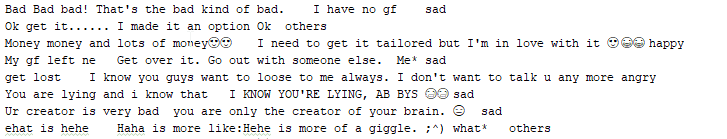
\includegraphics[width=\linewidth,height=5cm]{images/exemples_text}

En effet, on peut voir que certains mots sont inventés, d'autres mal écrits et certains sont des abbréviations. De plus, on voit que certains mots ne sont pas bien séparés par des espaces ce qui fait en sorte que ces algorithmes ne parviendraient pas bien à les séparer. Également, on souhaite limiter le temps de calcul pour l'optimisation de nos hyper-paramètres qui est déjà assez important.

Pour ces raisons, nous avons décidé de ne pas faire de stemming ou de lemmatisation sur nos données textuelles puisque nous jugeons que ces techniques n'apporteraient pas de gains de performance significatifs.

En conclusion, la matrice de données utilisée pour nos modèles de classification sera composée de données d'un des 3 objets de compte décrits dans cette sous-section avec ou sans les attributs supplémentaires décrits dans la section \nameref{sec:analyse_prelim} (si \verb|bool_ajouter_autres_features=True|).